\vspace{2mm}
\tikzset{every picture/.style={line width=0.75pt}} %set default line width to 0.75pt        

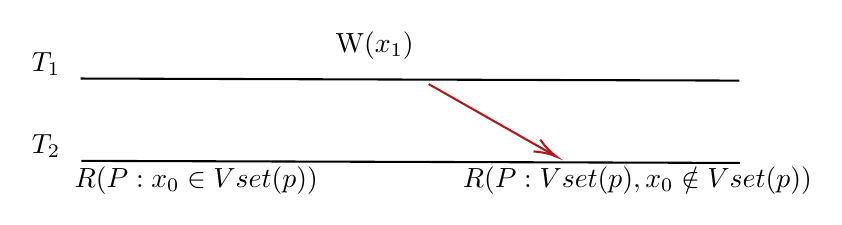
\begin{tikzpicture}[x=0.75pt,y=0.75pt,yscale=-1,xscale=1]
%uncomment if require: \path (0,300); %set diagram left start at 0, and has height of 300

%Straight Lines [id:da9351620672631715] 
\draw    (41.33,82) -- (358.67,83) ;
%Straight Lines [id:da20316716985592453] 
\draw    (41.67,121.67) -- (359,122.67) ;
%Straight Lines [id:da3663864520178606] 
\draw [color={rgb, 255:red, 179; green, 23; blue, 23 }  ,draw opacity=1 ]   (209,84.67) -- (268.93,118.68) ;
\draw [shift={(270.67,119.67)}, rotate = 209.58] [color={rgb, 255:red, 179; green, 23; blue, 23 }  ,draw opacity=1 ][line width=0.75]    (10.93,-3.29) .. controls (6.95,-1.4) and (3.31,-0.3) .. (0,0) .. controls (3.31,0.3) and (6.95,1.4) .. (10.93,3.29)   ;

% Text Node
\draw (16.33,68) node [anchor=north west][inner sep=0.75pt]   [align=left] {$T_1$};
% Text Node
\draw (16.33,107.33) node [anchor=north west][inner sep=0.75pt]   [align=left] {$T_2$};
% Text Node
\draw (162.67,58) node [anchor=north west][inner sep=0.75pt]   [align=left] {W($x_1$)};
% Text Node
\draw (224,123) node [anchor=north west][inner sep=0.75pt]   [align=left] {$R(P:Vset(p),x_0\notin Vset(p)$)};
% Text Node
\draw (37,123) node [anchor=north west][inner sep=0.75pt]   [align=left] {$R( P:x_0 \in Vset(p))$};


\end{tikzpicture}
\vspace{2mm}